\documentclass{article}
\usepackage[margin=1in]{geometry}
\usepackage{amsmath,amsthm,amssymb}
\usepackage{bbm,enumerate,mathtools}
\usepackage{tikz,pgfplots}
\usepackage{chessboard}
\usepackage[hidelinks]{hyperref}
\usepackage{multicol} % Problem 35
\usepackage{xstring} % Difficulty command
\usetikzlibrary{shapes.geometric}

\newenvironment{question}{\begin{trivlist}\item[\textbf{Question.}]}{\end{trivlist}}
\newenvironment{note}{\begin{trivlist}\item[\textbf{Note.}]}{\end{trivlist}}
\newenvironment{references}{\begin{trivlist}\item[\textbf{References.}]}{\end{trivlist}}
\newenvironment{related}{\begin{trivlist}\item[\textbf{Related.}]\end{trivlist}\begin{enumerate}}{\end{enumerate}}

\newcommand\score[1]{
\pgfmathsetmacro\pgfxa{#1+1}
\tikzstyle{scorestars}=[
  star,
  star points=5,
  star point ratio=2.25,
  draw,
  inner sep=3pt,
  anchor=outer point 5
]
  \begin{tikzpicture}[baseline]
    \draw[opacity=0] (0,-0.5) rectangle (0,0.2); % Workaround for whitespace at the bottom.
    \foreach \i in {1,...,4} {
      \pgfmathparse{(\i<=#1?"yellow":"gray")}
      \edef\starcolor{\pgfmathresult}
      \draw (\i*4.5ex,0) node[name=star\i,scorestars,fill=\starcolor]  {};
    }
  \end{tikzpicture}
}

\newcommand{\difficulty}[1]{%
  \IfEqCase{#1}{%
      {1}{
        
\begin{tikzpicture}[scale=0.7, baseline=0.9mm]%
          \definecolor{slopegreen}{rgb}{0.0, 0.5, 0.0}%
          \fill[slopegreen] (0.5,0.5) circle (0.5);%
        \end{tikzpicture}%
      }%
      {2}{
        
\begin{tikzpicture}[scale=0.7, baseline=0.9mm]%
          \definecolor{slopeblue}{rgb}{0.0, 0.44, 1.00}
          \fill[slopeblue] (0,0) rectangle (1,1);%
        \end{tikzpicture}%
      }%
      {3}{
\begin{tikzpicture}[scale=0.7, baseline=0.9mm]\fill (0,0.5)--(0.5, 0)--(1,0.5)--(0.5,1)--cycle; \end{tikzpicture}}%
      {4}{
\begin{tikzpicture}[scale=0.7, baseline=0.9mm]\fill (0.25,0)--(0,0.5)--(0.25,1)--(0.5,0.5)--cycle; \fill (0.75,0)--(0.5,0.5)--(0.75,1)--(1,0.5)--cycle;\end{tikzpicture}}%
      % you can add more cases here as desired
  }[\PackageError{difficulty}{Undefined difficulty level: #1}{}]%
}%
\newcommand{\rating}[2]{\difficulty{#1}\\\score{#2}\\}


\begin{document}

\rating{3}{2}
Consider maximal non-self-intersecting polygonal chains on $[n] \times [m]$
stable under $180^\circ$ rotation.

\begin{figure}[ht!]
  \centering
  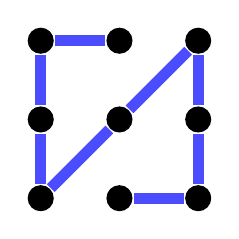
\begin{tikzpicture}
    \foreach \i in {1,2,3} {
      \foreach \j in {1,2,3} {
        \node[shape=circle, fill, thick] (v\i\j) at ({\j-1},{3-\i}) {};
      }
    }
    \draw[line width=4, blue!70]
      (v12) edge (v11)
      (v11) edge (v21)
      (v21) edge (v31)
      (v31) edge (v22)
      (v22) edge (v13)
      (v13) edge (v23)
      (v23) edge (v33)
      (v33) edge (v32)
    ;
  \end{tikzpicture}
  ~~~
  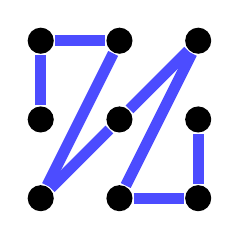
\begin{tikzpicture}
    \foreach \i in {1,2,3} {
      \foreach \j in {1,2,3} {
        \node[shape=circle, fill, thick] (v\i\j) at ({\j-1},{3-\i}) {};
      }
    }
    \draw[line width=4, blue!70]
      (v21) edge (v11)
      (v11) edge (v12)
      (v12) edge (v31)
      (v31) edge (v22)
      (v22) edge (v13)
      (v13) edge (v32)
      (v32) edge (v33)
      (v33) edge (v23)
    ;
  \end{tikzpicture}
  ~~~
  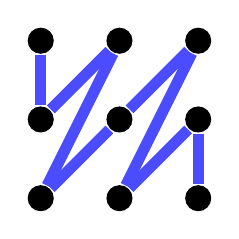
\begin{tikzpicture}
    \foreach \i in {1,2,3} {
      \foreach \j in {1,2,3} {
        \node[shape=circle, fill, thick] (v\i\j) at ({\j-1},{3-\i}) {};
      }
    }
    \draw[line width=4, blue!70]
      (v11) edge (v21)
      (v21) edge (v12)
      (v12) edge (v31)
      (v31) edge (v22)
      (v22) edge (v13)
      (v13) edge (v32)
      (v32) edge (v23)
      (v23) edge (v33)
    ;
  \end{tikzpicture}
  ~~~
  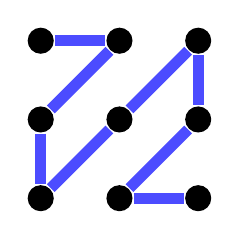
\begin{tikzpicture}
    \foreach \i in {1,2,3} {
      \foreach \j in {1,2,3} {
        \node[shape=circle, fill, thick] (v\i\j) at ({\j-1},{3-\i}) {};
      }
    }
    \draw[line width=4, blue!70]
      (v11) edge (v12)
      (v12) edge (v21)
      (v21) edge (v31)
      (v31) edge (v22)
      (v22) edge (v13)
      (v13) edge (v23)
      (v23) edge (v32)
      (v32) edge (v33)
    ;
  \end{tikzpicture}
  \\~\\
  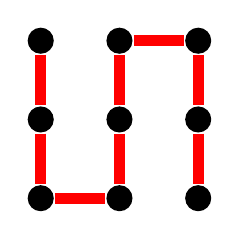
\begin{tikzpicture}
    \foreach \i in {1,2,3} {
      \foreach \j in {1,2,3} {
        \node[shape=circle, fill, thick] (v\i\j) at ({\j-1},{3-\i}) {};
      }
    }
    \draw[line width=4, red]
      (v11) edge (v21)
      (v21) edge (v31)
      (v31) edge (v32)
      (v32) edge (v22)
      (v22) edge (v12)
      (v12) edge (v13)
      (v13) edge (v23)
      (v23) edge (v33)
    ;
  \end{tikzpicture}
  ~~~
  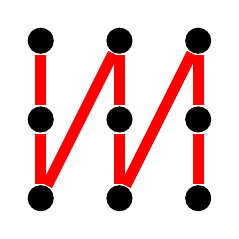
\begin{tikzpicture}
    \foreach \i in {1,2,3} {
      \foreach \j in {1,2,3} {
        \node[shape=circle, fill, thick] (v\i\j) at ({\j-1},{3-\i}) {};
      }
    }
    \draw[line width=4, red]
      (v11) edge (v21)
      (v21) edge (v31)
      (v31) edge (v12)
      (v12) edge (v22)
      (v22) edge (v32)
      (v32) edge (v13)
      (v13) edge (v23)
      (v23) edge (v33)
    ;
  \end{tikzpicture}
  ~~~
  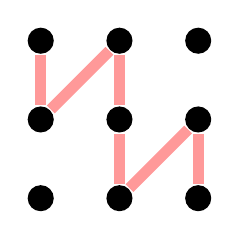
\begin{tikzpicture}
    \foreach \i in {1,2,3} {
      \foreach \j in {1,2,3} {
        \node[shape=circle, fill, thick] (v\i\j) at ({\j-1},{3-\i}) {};
      }
    }
    \draw[line width=4, red!40]
      (v11) edge (v21)
      (v21) edge (v12)
      (v12) edge (v22)
      (v22) edge (v32)
      (v32) edge (v23)
      (v23) edge (v33)
    ;
  \end{tikzpicture}
  ~~~
  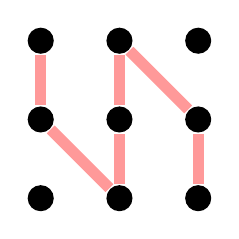
\begin{tikzpicture}
    \foreach \i in {1,2,3} {
      \foreach \j in {1,2,3} {
        \node[shape=circle, fill, thick] (v\i\j) at ({\j-1},{3-\i}) {};
      }
    }
    \draw[line width=4, red!40]
      (v11) edge (v21)
      (v21) edge (v32)
      (v32) edge (v22)
      (v22) edge (v12)
      (v12) edge (v23)
      (v23) edge (v33)
    ;
  \end{tikzpicture}
  \caption{The $6$ (or $8$) maximal polygonal chains with vertices in $[3] \times [3]$.}
\end{figure}

\begin{question}
  How many non-self-intersecting polygonal chains with vertex set equal to
  $[n] \times [m]$ are stable under $180^\circ$ rotation?
\end{question}

\begin{related}
  \item What if this is done with other kinds of symmetry?
  (e.g. horizontal or vertical reflection)
  \item What if this is done for polygons instead of polygonal chains?
  \item What if maximal means that the polygonal chain cannot be extended, a
  weaker condition than that the vertex set is $[n] \times [m]$.
  (This includes the last two chains in the example.)
  \item What is the maximal length of such a chain with respect to
    $\ell_1, \ell_2,$ and $\ell_\infty$?
    What if the symmetry restriction is dropped?
  \item What if the only allowed moves are king moves? Rook moves?
  \item What if this is done with vertex set
    $[n_1] \times [n_2] \times \cdots \times [n_k]$?
\end{related}

\begin{references}
  \item Problems 5, 44, 46, 55, 68, 74, 87, and 104.
\end{references}
\end{document}
